\documentclass[12pt]{beamer}
\usepackage{booktabs}
\beamertemplatenavigationsymbolsempty
\AtBeginSection[]
{
    \begin{frame}
    \frametitle{Table of Contents}
    \tableofcontents[currentsection]
    \end{frame}
}

\title{Graph basics}
\subtitle{Definitions, representations}
\author{beOI Training}
\institute{
\includegraphics[height=12em]{img/beoi-logo}}

\begin{document}

\frame{\titlepage}

\section{Introduction to graphs}

\begin{frame}
\frametitle{Graphs, intuitively}
\begin{itemize}
\item Points (vertex, nodes)
\item Lines between the points (edges, links)
\end{itemize}
\begin{figure}
\centering
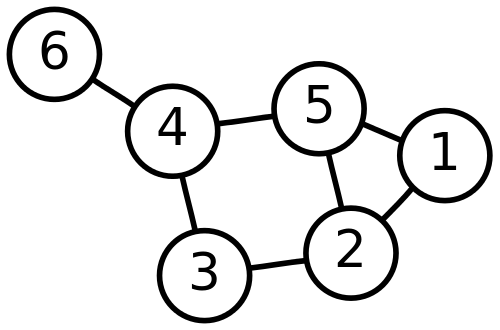
\includegraphics[width=0.5\linewidth]{img/6n-graph}
\end{figure}
\end{frame}

\begin{frame}
\frametitle{Graphs, mathematically}
\[ \mathbf{G}\mathsf{raph} = (\mathbf{V}\mathsf{ertices}, \mathbf{E}\mathsf{dges}) \]
\begin{figure}
\centering
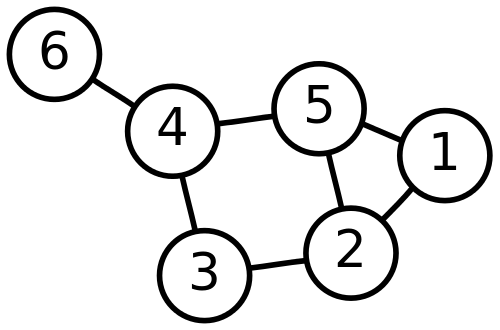
\includegraphics[width=0.5\linewidth]{img/6n-graph}
\end{figure}
\[ V= \{1,2,3,4,5,6\} \]
\[ E= \{(1,2),(1,5),(2,3),(2,5),(3,4),(4,5),(4,6)\} \]
\end{frame}

\begin{frame}
\frametitle{Terminology}
\begin{itemize}
\item $u$ and $v$ adjacent $\Leftrightarrow (u,v) \in E$
\item Degree of $u = \#\{\mbox{edges from }u\}$
\end{itemize}
\begin{figure}
\centering
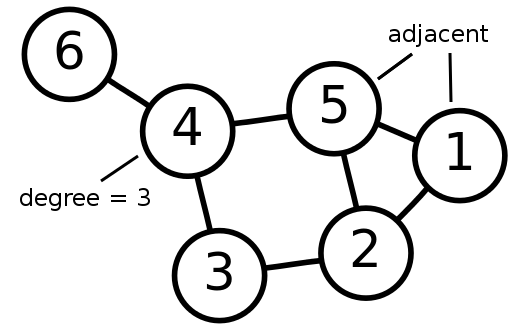
\includegraphics[width=0.6\linewidth]{img/6n-graph-term}
\end{figure}
\end{frame}

\begin{frame}
\frametitle{Simple graph vs multigraph}
\begin{figure}
\centering
\setlength{\tabcolsep}{10pt}
\begin{tabular}{cc}
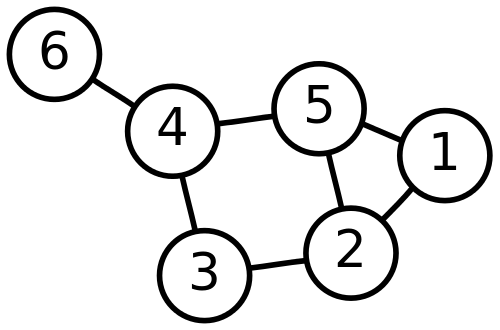
\includegraphics[width=0.4\linewidth]{img/6n-graph}
& 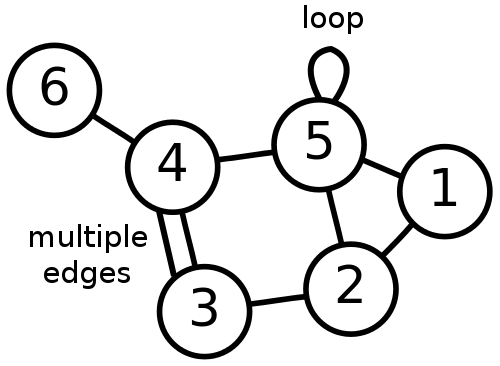
\includegraphics[width=0.4\linewidth]{img/6n-multi} \\
simple graph & multigraph
\end{tabular}
\end{figure}
\end{frame}

\begin{frame}
\frametitle{Directed vs undirected}
\begin{figure}
\centering
\begin{tabular}{cc}
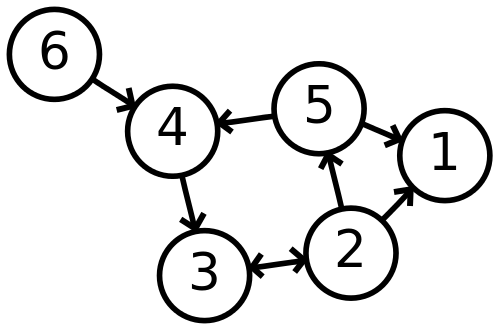
\includegraphics[width=0.4\linewidth]{img/6n-directed}
& 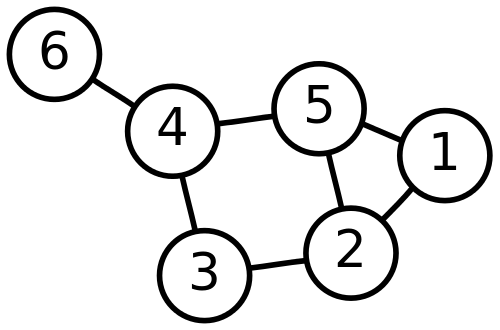
\includegraphics[width=0.4\linewidth]{img/6n-graph} \\
directed & undirected
\end{tabular}
\end{figure}
\end{frame}

\begin{frame}
\frametitle{Weighted vs unweighted}
\begin{itemize}
\item Represent costs, times, lengths, capacities
\end{itemize}
\begin{figure}
\centering
\begin{tabular}{cc}
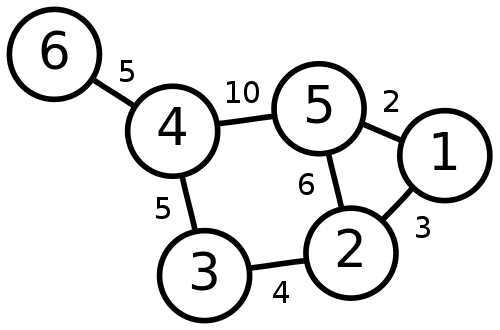
\includegraphics[width=0.4\linewidth]{img/6n-weighted}
& 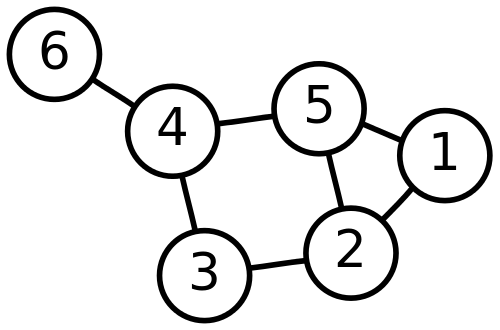
\includegraphics[width=0.4\linewidth]{img/6n-graph} \\
weighted & unweighted
\end{tabular}
\end{figure}
\end{frame}

\begin{frame}
\frametitle{Paths and cycles}
\begin{itemize}
\item $u$ and $v$ connected $\Leftrightarrow$ path $u \to v$
\item $G$ connected $\Leftrightarrow$ all pairs connected
\end{itemize}
\begin{figure}
\centering
\begin{tabular}{cc}
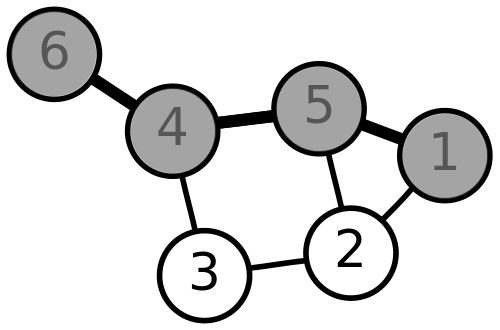
\includegraphics[width=0.4\linewidth]{img/6n-path}
& 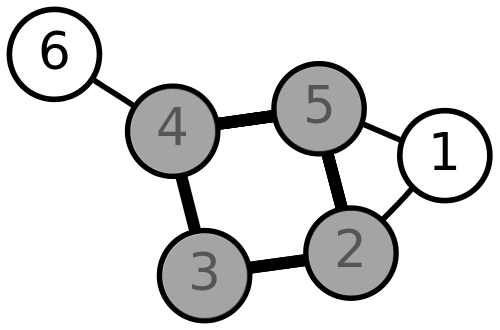
\includegraphics[width=0.4\linewidth]{img/6n-cycle} \\
path & cycle
\end{tabular}
\end{figure}
\end{frame}

\begin{frame}
\frametitle{Trees}
\begin{columns}[c]
\column{.3\linewidth}
\begin{itemize}
\item Connected
\item Acyclic
\item $|E| = |V|-1$
\end{itemize}
\column{.7\linewidth}
\centering
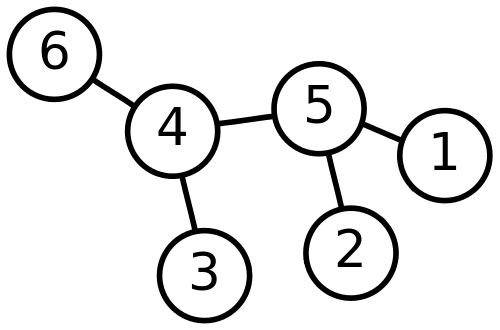
\includegraphics[width=0.7\linewidth]{img/6n-tree}
\end{columns}
\end{frame}

\section{Graph representation}

\begin{frame}
\frametitle{Edge list}
\begin{itemize}
\item Vector of pairs: \texttt{vector<pair<int,int>> edges}
\item Same as input / mathematical definition
\item Limited use (only Kruskal)
\end{itemize}
\begin{figure}
\centering
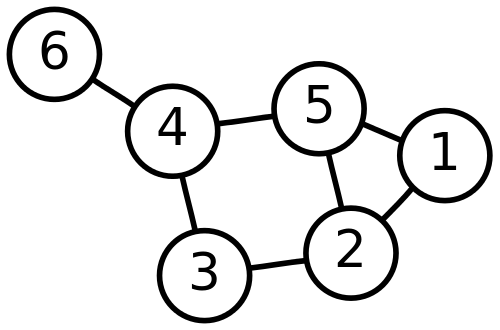
\includegraphics[width=0.5\linewidth]{img/6n-graph}
\end{figure}
\begin{center}
\texttt{edges[]}$ = \{(1,2),(1,5),(2,3),(2,5),(3,4),(4,5),(4,6)\}$
\end{center}
\end{frame}

\begin{frame}
\frametitle{Adjacency matrix on undirected graph}
\begin{itemize}
\item Static two-dimensional array: \texttt{bool adj[MAXN][MAXN]}
\item \texttt{adj[i][j] == true} if edge $i \to j$
\item Symmetric
\end{itemize}
\begin{columns}
\column{.5\linewidth}
\flushright
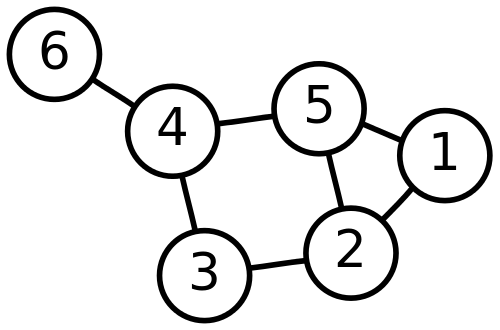
\includegraphics[width=0.85\linewidth]{img/6n-graph}
\column{.5\linewidth}
\[\left(
\begin{array}{cccccc}
0&1&0&0&1&0\\
1&0&1&0&1&0\\
0&1&0&1&0&0\\
0&0&1&0&1&1\\
1&1&0&1&0&0\\
0&0&0&1&0&0\\
\end{array}
\right)\]
\end{columns}
\end{frame}

\begin{frame}
\frametitle{Adjacency matrix on directed graph}
\begin{itemize}
\item Only put \texttt{true} in one direction
\item Not symmetric
\end{itemize}
\begin{columns}
\column{.5\linewidth}
\flushright
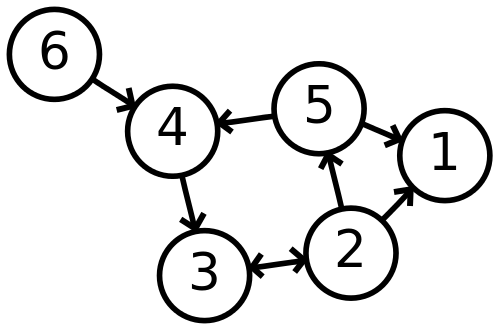
\includegraphics[width=0.85\linewidth]{img/6n-directed}
\column{.5\linewidth}
\[\left(
\begin{array}{cccccc}
0&0&0&0&0&0\\
1&0&1&0&1&0\\
0&1&0&0&0&0\\
0&0&1&0&0&0\\
1&0&0&1&0&0\\
0&0&0&1&0&0\\
\end{array}
\right)\]
\end{columns}
\end{frame}

\begin{frame}
\frametitle{Adjacency matrix on weighted graph}
\begin{itemize}
\item Change the type: \texttt{int adj[MAXN][MAXN]}
\item Instead of \texttt{true} put the weights
\end{itemize}
\begin{columns}
\column{.5\linewidth}
\flushright
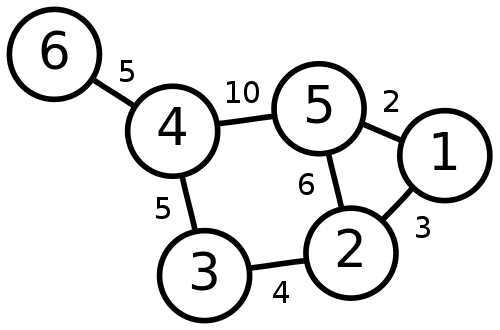
\includegraphics[width=0.85\linewidth]{img/6n-weighted}
\column{.5\linewidth}
\[\left(
\begin{array}{cccccc}
0&3&0&0&2&0\\
3&0&4&0&6&0\\
0&4&0&5&0&0\\
0&0&5&0&10&5\\
2&6&0&10&0&0\\
0&0&0&5&0&0\\
\end{array}
\right)\]
\end{columns}
\end{frame}

\begin{frame}
\frametitle{Adjacency list on undirected graph}
\begin{itemize}
\item Array of vectors: \texttt{vector<int> neigh[MAXN]}
\item For each vertex, list the neighbors
\end{itemize}
\begin{columns}
\column{.6\linewidth}
\flushright
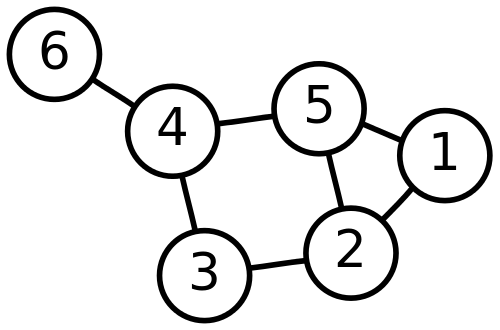
\includegraphics[width=0.75\linewidth]{img/6n-graph}
\column{.4\linewidth}
\begin{enumerate}
\item $\{2,5\}$
\item $\{1,3,5\}$
\item $\{2,4\}$
\item $\{3,5,6\}$
\item $\{1,2,4\}$
\item $\{4\}$
\end{enumerate}
\end{columns}
\end{frame}

\begin{frame}
\frametitle{Adjacency list on directed graph}
\begin{itemize}
\item Only list in one direction
\end{itemize}
\begin{columns}
\column{.6\linewidth}
\flushright
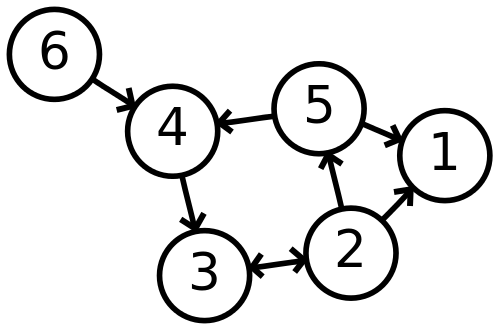
\includegraphics[width=0.75\linewidth]{img/6n-directed}
\column{.4\linewidth}
\begin{enumerate}
\item $\{\}$
\item $\{1,3,5\}$
\item $\{2\}$
\item $\{3\}$
\item $\{1,4\}$
\item $\{4\}$
\end{enumerate}
\end{columns}
\end{frame}

\begin{frame}
\frametitle{Adjacency list on weighted graph}
\begin{itemize}
\item Add the weight lists: \texttt{vector<int> weight[MAXN]}
\end{itemize}
\begin{columns}
\column{.45\linewidth}
\flushright
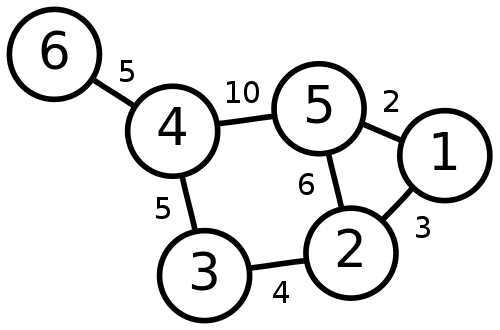
\includegraphics[width=0.8\linewidth]{img/6n-weighted}
\column{.25\linewidth}
\texttt{neigh[]}
\begin{enumerate}
\item $\{2,5\}$
\item $\{1,3,5\}$
\item $\{2,4\}$
\item $\{3,5,6\}$
\item $\{1,2,4\}$
\item $\{4\}$
\end{enumerate}
\column{.3\linewidth}
\texttt{weight[]}
\begin{enumerate}
\item $\{3,2\}$
\item $\{3,4,6\}$
\item $\{4,5\}$
\item $\{5,10,5\}$
\item $\{2,6,10\}$
\item $\{5\}$
\end{enumerate}
\end{columns}
\end{frame}

\begin{frame}
\frametitle{Comparison}
\begin{itemize}
\item Use adjacency list (most of the time)
\item Adjacency matrix only used for fast edge lookup
\end{itemize}
\begin{figure}
\centering
\begin{tabular}{rccc}
& Size & List all edges & Edge lookup \\
\midrule
\multicolumn{1}{r|}{Matrix} & $O(V^2)$ & $O(V^2)$ & $O(1)$ \\
\multicolumn{1}{r|}{List} & $O(V+E)$ & $O(V+E)$ & $O(\mathsf{deg}(u))$
\end{tabular}
\end{figure}
\end{frame}

\begin{frame}
\frametitle{Tree, parent representation}
\begin{itemize}
\item Choose a root
\item Every node has a parent (except the root)
\item Parents lead to the root
\end{itemize}
\begin{figure}
\centering
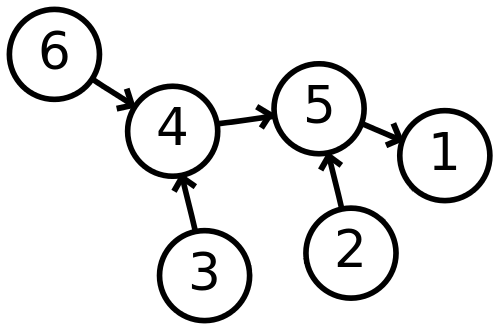
\includegraphics[width=.5\linewidth]{img/6n-tree-parent}
\end{figure}
\begin{center}
\texttt{parent[]} = $\{-,5,4,5,1,4\}$
\end{center}
\end{frame}

\begin{frame}
\frametitle{Tree, child representation}
\begin{itemize}
\item For each node, list the children
\item Nodes 2, 3, 6 are leaves (no children)
\end{itemize}
\begin{columns}
\column{.6\linewidth}
\flushright
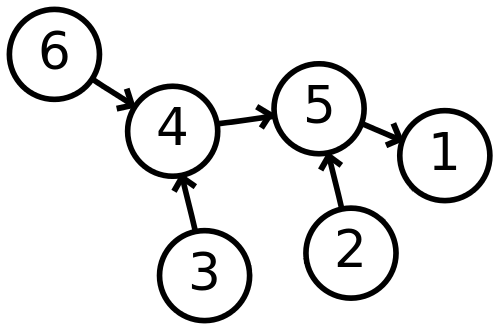
\includegraphics[width=0.75\linewidth]{img/6n-tree-parent}
\column{.4\linewidth}
\begin{enumerate}
\item $\{5\}$
\item $\{\}$
\item $\{\}$
\item $\{3,6\}$
\item $\{2,4\}$
\item $\{\}$
\end{enumerate}
\end{columns}
\end{frame}

\begin{frame}
\frametitle{Source of figures}
\begin{itemize}
\item \url{https://en.wikipedia.org/wiki/File:6n-graf.svg}
\end{itemize}
\end{frame}

\end{document}
